\documentclass[11pt,a4paper]{article}

\usepackage[utf8]{inputenc}
\usepackage[T1]{fontenc}
\usepackage[english]{babel}
\usepackage{amsmath,amssymb,mathtools}
\usepackage{geometry}
\geometry{margin=1in}
\usepackage{fancyhdr}
\usepackage{titlesec}
\usepackage{tikz}

\pagestyle{fancy}
\fancyhf{}
\fancyhead[C]{\small Cayley --- Collected Mathematical Papers, Vol.\ VIII}
\fancyfoot[C]{\thepage}
\renewcommand{\headrulewidth}{0.4pt}

\titleformat{\section}{\large\scshape\centering}{}{0em}{}
\titleformat{\subsection}{\normalsize\bfseries\centering}{}{0em}{}

\newcommand{\sourcepage}[3]{%
  \bigskip
  \noindent\textit{p.~#1 [#2]; source scan p.~#3}%
  \par\smallskip
}
\newcommand{\oproduct}[1]{\overline{#1}}

\newcommand{\signsquareone}{%
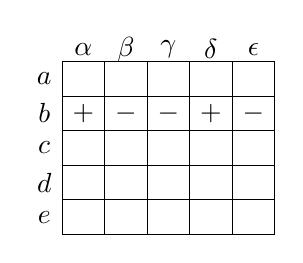
\begin{tikzpicture}[baseline=(current bounding box.center), x=0.54cm, y=0.44cm]
  \foreach \i in {0,...,5} {
    \draw[line width=0.3pt] (\i,0) -- (\i,5);
    \draw[line width=0.3pt] (0,\i) -- (5,\i);
  }
  \node at (-0.42,4.5) {$a$};
  \node at (-0.42,3.5) {$b$};
  \node at (-0.42,2.5) {$c$};
  \node at (-0.42,1.5) {$d$};
  \node at (-0.42,0.5) {$e$};
  \node at (0.5,5.35) {$\alpha$};
  \node at (1.5,5.35) {$\beta$};
  \node at (2.5,5.35) {$\gamma$};
  \node at (3.5,5.35) {$\delta$};
  \node at (4.5,5.35) {$\epsilon$};
  \node at (0.5,3.5) {$+$};
  \node at (1.5,3.5) {$-$};
  \node at (2.5,3.5) {$-$};
  \node at (3.5,3.5) {$+$};
  \node at (4.5,3.5) {$-$};
\end{tikzpicture}%
}

\newcommand{\signsquaretwo}{%
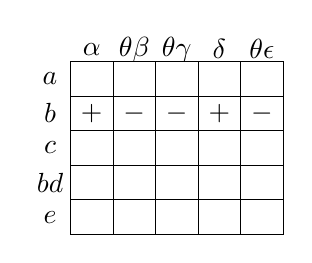
\begin{tikzpicture}[baseline=(current bounding box.center), x=0.54cm, y=0.44cm]
  \foreach \i in {0,...,5} {
    \draw[line width=0.3pt] (\i,0) -- (\i,5);
    \draw[line width=0.3pt] (0,\i) -- (5,\i);
  }
  \node at (-0.48,4.5) {$a$};
  \node at (-0.48,3.5) {$b$};
  \node at (-0.48,2.5) {$c$};
  \node at (-0.48,1.5) {$bd$};
  \node at (-0.48,0.5) {$e$};
  \node at (0.5,5.35) {$\alpha$};
  \node at (1.5,5.35) {$\theta\beta$};
  \node at (2.5,5.35) {$\theta\gamma$};
  \node at (3.5,5.35) {$\delta$};
  \node at (4.5,5.35) {$\theta\epsilon$};
  \node at (0.5,3.5) {$+$};
  \node at (1.5,3.5) {$-$};
  \node at (2.5,3.5) {$-$};
  \node at (3.5,3.5) {$+$};
  \node at (4.5,3.5) {$-$};
\end{tikzpicture}%
}

\newcommand{\diagonalsquare}{%
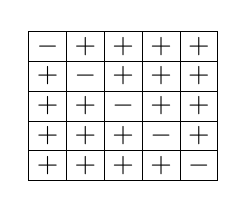
\begin{tikzpicture}[baseline=(current bounding box.center), x=0.48cm, y=0.38cm]
  \foreach \i in {0,...,5} {
    \draw[line width=0.3pt] (\i,0) -- (\i,5);
    \draw[line width=0.3pt] (0,\i) -- (5,\i);
  }
  \foreach \r in {0,...,4} {
    \foreach \c in {0,...,4} {
      \pgfmathtruncatemacro{\same}{ifthenelse(\r==\c,1,0)}
      \ifnum\same=1
        \node at (\c+0.5,4.5-\r) {$-$};
      \else
        \node at (\c+0.5,4.5-\r) {$+$};
      \fi
    }
  }
\end{tikzpicture}%
}

\begin{document}

% ============================================================
% PAPER 545
% ============================================================
\sourcepage{529}{545}{593}
\section{[545]}
\subsection{On the Theory of the Singular Solutions of Differential Equations of the First Order.}

\begin{center}
\textit{[From the Messenger of Mathematics, vol.~\textsc{ii}. (1873), pp.~6---12.]}
\end{center}

\textsc{I consider} a differential equation under the form
\[
\phi(x,y,p)=0,
\]
where

\begin{enumerate}
\item[$1^\circ$.] $\phi$ is as to $p$, rational and integral of the degree $n$;
\item[$2^\circ$.] it is, or is taken to be, one-valued in regard to $(x,y)$;
\item[$3^\circ$.] it has no mere $(x,y)$ factor;
\item[$4^\circ$.] it is indecomposable as regards $p$.
\end{enumerate}

Considering $(x,y)$ as the coordinates of a point \textit{in plano}, the differential equation
determines a system of curves, in general indecomposable, the system depending on
a single variable parameter, and such that through each point of the plane there pass
$n$ curves.

Such a system is represented by an integral equation
\[
f(x,y,c_1,c_2,\ldots,c_m)=0,
\]
where

\begin{enumerate}
\item[$5^\circ$.] $f$ is rational and integral in regard to the $m$ constants, which constants are
connected by an algebraic $(m-1)$ fold relation;
\item[$6^\circ$.] it is, or is taken to be, one-valued in regard to $(x,y)$;
\item[$7^\circ$.] it has no mere $(x,y)$ factor;
\item[$8^\circ$.] it is indecomposable as regards $(x,y)$;
\end{enumerate}

\clearpage

\sourcepage{530}{545}{594}
\begin{enumerate}
\item[$9^\circ$.] Considering $(x,y)$ as given, the equation $f=0$, together with the $(m-1)$ fold
relation between the constants, must constitute a $m$-fold relation of the order $n$, that is,
must give for the constants $n$ sets of values. We may, if we please, take $f$ to be
linear in regard to the constants $c_1,c_2,\ldots,c_m$, and then the condition simply is, that
the $(m-1)$ fold relation shall be of the order $n$.
\end{enumerate}

I give in regard to these definitions such explanations as seem necessary.

$2^\circ$. A one-valued function of $(x,y)$ is either a rational function, or a function
such as $e^x\sin y$, \&c., which for any given values whatever, real or imaginary, of the
variables, has only one value. A function is taken to be one-valued when, either for
any values whatever of the variables, or for any class of values (e.g. all real values),
we select for any given values of the variables one value, and attend exclusively to
such one value, of the function.

Thus, $U$ a rational function of $(x,y)$, $\phi=p^2-U=0$, $\phi$ is one-valued in regard to
$(x,y)$. But if, $U$ not being the square of a rational function, we take $\sqrt{U}$ to be
a one-valued function (consider it as denoting, say for all real values of $x,y$ for which
$U$ is positive, the positive square-root of $U$), then, $\phi=p+\sqrt{U}=0$, $\phi$ is taken
to be one-valued in regard to $(x,y)$.

$3^\circ$. The meaning is, that the equation $\phi=0$ is not satisfied irrespectively of the
value of $p$, by any relation between the variables $x,y$.

$4^\circ$. The meaning is that $\phi$ is not the product of two factors, each rational and
integral in regard to $p$, and being or being taken to be one-valued in regard to $(x,y)$.
Thus, if as before $U$ is a rational function of $(x,y)$ but is not the square of a
rational function, and if we do not take any one-valued function, then the equation
$\phi=p^2-U=0$ is indecomposable; but if we take $\sqrt{U}$ as one-valued, then we have
\[
\phi=\{p-\sqrt{U}\}\{p+\sqrt{U}\}=0,
\]
and the equation breaks up into the two equations
$p-\sqrt{U}=0$ and $p+\sqrt{U}=0$. I assume as an axiom, that the curves represented by
the indecomposable differential equation are in general indecomposable; for supposing the
differential equation satisfied in regard to a system of curves, the general curve breaking
into two curves, each depending on the arbitrary parameter, then we have two distinct
systems of curves; either the differential equation is satisfied in regard to each system
separately, and in this case they are the same system twice repeated; or the differential
equation is satisfied in regard to one system only, and in this case the other system
is not part of the solution, and it is to be rejected. As an instance, take the equation
$\phi=px+y=0$, $(x\,dy+y\,dx=0)$; if we choose to integrate this in the form $x^2y^2-c=0$,
this equation represents the two hyperbolas $xy+\sqrt{c}=0$, $xy-\sqrt{c}=0$, but considering
each of these separately, and giving to the constant $c$ any value whatever, we
have simply the system of hyperbolas $xy-c=0$ twice repeated. But if by any (faulty)
process of integration the solution had been obtained in a form such as $(c+x)(c-xy)=0$,
then the differential equation is not satisfied in regard to the system $c+x=0$; and
the factor $c+x$ is to be rejected. Observe that it is said, that the curves are \textit{in
general} indecomposable; particular curves of the system may very well be decomposable;
thus in the foregoing example, where the system of curves is $xy-c=0$, in the
particular case $c=0$, the hyperbola breaks up into the two lines $x=0$, $y=0$.

\clearpage

\sourcepage{531}{545}{595}
$5^\circ$. It is necessary to consider a form $f=0$ involving the $m$ constants connected
by the $(m-1)$ fold relation. For taking such a system of constants, imagine an
equation $f(x,y,c_1,c_2,\ldots,c_m)=0$ rational and integral in regard to $(x,y)$, and representing
an indecomposable curve; such an integral equation leads to a differential equation
of the form $\phi(x,y,p)=0$, rational in regard to $(x,y)$; whence, conversely, a differential
equation of the form last referred to may have for its integral the equation
$f(x,y,c_1,c_2,\ldots,c_m)=0$. And we cannot in a proper form exhibit this integral in terms
of a single constant. For first consider for a moment $c_1,c_2,\ldots,c_m$ as the coordinates
of a point in $m$-dimensional space; the curve is not in general unicursal, and unless
it be so, we cannot express the quantities $c_1,c_2,\ldots,c_m$ rationally in terms of a parameter;
that is, we cannot in general express $c_1,c_2,\ldots,c_m$ rationally in terms of a
parameter. Secondly, if by means of the $(m-1)$ fold relation we sought to eliminate
from the equation $f=0$ all but one of the $m$ constants, we should indeed arrive at
an equation $F(x,y,c)=0$ rational and integral as regards $x$ and $y$, and also as regards
$c$; but this equation would not represent an indecomposable curve.

$6^\circ$. It is important to remark that, even in the case where $\phi(x,y,p)$ is one-valued
in regard to $(x,y)$ ($2^\circ$), there is not in every case a form $f=0$ one-valued
in regard to $(x,y)$. A simple example shows this; let $\alpha,\beta$ be incommensurable
(e.g. $\alpha=e$, $\beta=\pi$), then the equation $\phi=\beta xp+\alpha y=0$ $(\alpha y\,dx+\beta x\,dy=0)$ has for its
integral $c=x^\alpha y^\beta$, where $x^\alpha y^\beta$ is not a one-valued function of $x,y$, and we cannot in
any way whatever transform the integral so as to express it in terms of one-valued
functions of $x$ and $y$. But taking $x^\alpha y^\beta$ to be a one-valued function---if e.g. for all
real values of $x,y$ we consider $x^\alpha y^\beta$ as representing the real value of $(\pm x)^\alpha(\pm y)^\beta$---,
we shall have, without any loss of generality, the integral of the differential equation;
the whole system of curves $c=x^\alpha y^\beta$, $c$ any value whatever, is the same whether we
attribute to $x^\alpha y^\beta$ its infinite series of values, or only one of these values.

$7^\circ$. The meaning is, that the equation $f=0$ is not satisfied irrespectively of the
values of $c_1,c_2,\ldots,c_m$ by any relation between $x,y$ only.

$8^\circ$. The meaning is, that the function $f$ is not the product of two factors, rational
or irrational in regard to $c_1,c_2,\ldots,c_m$, but each of them one-valued or taken to be
one-valued in regard to $x,y$. Thus the function
\[
f=x^2y^2-c,\qquad =\{xy+\sqrt{c}\}\{xy-\sqrt{c}\},
\]
is decomposable; but if we do not take any one-valued function, then $f=xy-c$ is
indecomposable; if we take $\sqrt{xy}$ to be one-valued, then it is decomposable.

The case $f=x^\alpha y^\beta-c$ ($\alpha$ and $\beta$ incommensurable) is to be noticed; starting from
the differential equation $\alpha y\,dx+\beta x\,dy=0$, there is no reason for writing the integral
\[
\begin{gathered}
f=x^\alpha y^\beta-c=0,\\
\text{rather than in either of the forms}\\
f=x^{m\alpha}y^{m\beta}-c=0,\qquad
f=x^{\frac{\alpha}{m}}y^{\frac{\beta}{m}}-c=0,
\end{gathered}
\]
($m$ an integer), $(\alpha,\beta)$, $(m\alpha,m\beta)$, $\left(\frac{\alpha}{m},\frac{\beta}{m}\right)$ are,
each pair as well as the others, two incommensurable magnitudes. If we choose to take
$x^\alpha y^\beta$ but not $x^{\frac{\alpha}{m}}y^{\frac{\beta}{m}}$ as one-valued,

\clearpage

\sourcepage{532}{545}{596}
then $f=x^\alpha y^\beta-c$ and $f=x^{m\alpha}y^{m\beta}-c$ are each one-valued, and the former is, the latter
is not, indecomposable; they would be each decomposable if we chose to take
$x^{\frac{\alpha}{m}}y^{\frac{\beta}{m}}$ as one-valued; and if only $x^{m\alpha}y^{m\beta}$ were taken to be
one-valued, then $f=x^{m\alpha}y^{m\beta}-c$ would be indecomposable.

$9^\circ$. This is a mere statement of the condition in order that the system of curves
represented by the integral equation may be such that, through a given point of the
plane, there may pass $n$ of these curves. Since the number of constants is unlimited,
there is clearly no loss of generality in assuming that the equation is linear in regard
to the several constants.

I consider now the differential equation
\[
\phi(x,y,p)=0,
\]
(as already stated of the degree $n$ as regards $p$), and its integral equation
\[
f(x,y,c_1,c_2,\ldots,c_m)=0.
\]
I take $(x,y)$ to be the coordinates of a point, say in the horizontal plane, and I use
$C$ to refer to the constants $c_1,c_2,\ldots,c_m$ collectively, thus for given values of $x,y$ I speak
of the $n$ values of $C$, meaning thereby the $n$ values of the set $(c_1,c_2,\ldots,c_m)$; of $C$
having a two-fold value, meaning thereby that two of the sets $c_1,c_2,\ldots,c_m$ become
identical; and so on.

The case $C=c$, where there is only a single constant $c$, is interesting as affording
an easier geometrical conception; we may take $c=z$ to be a third coordinate; the
equation $f(x,y,z)=0$ thus represents a surface, such that its plane sections $z=c$, or
say these sections projected by vertical ordinates on the horizontal plane $z=0$ are the
series of curves $f(x,y,c)=0$. But the case is not really distinct from the general one.

The theory of singular solutions depends on the following considerations:

To a given point $P$ on the horizontal plane belong $n$ values of $C$, each determining
a curve $f(x,y,C)=0$ through $P$; and also $n$ values of $p$, viz. these give the
directions at $P$ of the $n$ curves respectively.

The curve $f(x,y,C)=0$ may be such as to have in general a certain number
of nodes and of cusps (either or each of these numbers being $=0$): we may imagine $C$
determined, say $C=C_0$, so that the curve shall have one additional node: this node I
call a ``level point.'' Take $P$ at the level point, there are $n$ values of $C$, viz. $C_0$ and
$n-1$ other values; that is, there are through $P$ the nodal curve, and $n-1$ other
curves, and therefore $2+(n-1)$, $=n+1$ directions of the tangent; but the directions
are determined by the equation $\phi=0$ of the order $n$: and the only way in which
we can have more than $n$ values is when this equation becomes an identity $0=0$;
that is, $P$ at the level point, the function $\phi(x,y,p)$ will vanish identically, irrespectively
of the value of $p$.

\clearpage

\sourcepage{533}{545}{597}
The ordinary nodes (if any) on the curves $f(x,y,C)=0$ form a locus called the
``nodal locus,'' and the cusps (if any) a locus called the ``cuspidal locus.'' Take the
point $P$ a given point on the nodal locus, $C$ has a two-fold value answering to the
curve in regard to which $P$ is a node, and $n-2$ other values; that is, the $n$ curves
through $P$ are the nodal curve reckoned twice and $n-2$ other curves; the directions
are the directions at the node, and the $n-2$ other directions, in all $n$ directions, which
are the directions given by the equation $\phi=0$; there is no peculiarity in regard to
this equation.

Similarly, take $P$ anywhere on the cuspidal locus: $C$ has a two-fold value, answering
to the curve in regard to which $P$ is a cusp, and $n-2$ other values; that is, the
$n$ curves through $P$ are the cuspidal curve reckoned twice and $n-2$ other curves;
the directions are the direction at the cusp reckoned twice and $n-2$ other directions:
in all $n$ directions, which are the directions given by the equation $\phi=0$; this equation
thus gives a two-fold value of $p$.

There is a locus (distinct from the nodal and cuspidal loci) which may be called
the ``envelope locus,'' such that taking $P$ anywhere on this locus $C$ has a two-fold
value; for such position of $P$ the $n$ values of $C$ are the value in question reckoned
twice and $n-2$ other values; the $n$ curves through $P$ are that belonging to the
two-fold value of $C$, or say the two-fold curve, and $n-2$ other values; and the $n$
directions are the direction along the two-fold curve counted twice, and $n-2$ other
directions; these are the $n$ directions given by the equation $\phi=0$, viz. this equation
gives a two-fold value of $p$.

The envelope locus may be an indecomposable curve, or it may break up into
two or more curves; and it may happen that either the whole curve or one or more
of the component curves may coincide with a particular curve or curves of the system
$f(x,y,C)=0$.

There is a locus (distinct from the cuspidal and envelope loci) which may be
called the tac-locus, such that taking $P$ anywhere on this locus $p$ has a two-fold
value; for such position of $P$, there is no peculiarity as regards $C$, viz. $C$ has $n$
distinct values giving rise to $n$ curves through $P$; but as the directions are given
by the equation $\phi=0$, two of the curves touch each other, viz. the tac-locus is the
locus of points, such that at any one of them two of the curves $f(x,y,C)=0$ through
the point touch each other.

We may by an extension of the received notation write
\[
\operatorname{disc}_{C} f(x,y,C)=0
\]
to denote the equation between $(x,y)$, such that, for any values of $(x,y)$, which satisfy
the condition, or say for any position of $P$ on the $C$-discriminant locus, there is a
two-fold value of $C$. By what precedes it appears that the $C$-discriminant locus is
made up of the nodal, cuspidal, and envelope loci, and without going into the proof
I infer that it is in fact made up of the nodal locus twice, the cuspidal locus three
times, and the envelope locus once.

\clearpage

% ============================================================
% PAPER 545, final page in this slice
% ============================================================
\sourcepage{534}{545}{598}
\section{[545]}
\subsection{On Singular Solutions.}

Writing moreover
\[
\operatorname{disct}_{p}\,\phi(x,y,p)=0
\]
to denote the equation between $(x,y)$, such that for any values of $(x,y)$
which satisfy the condition, or say for any position of $P$ on the
$p$-discriminant locus, there is a two-fold value of $p$. By what precedes,
it appears that the $p$-discriminant locus is made up of the envelope locus,
cuspidal locus, and the tac-locus; as I infer, each of them once.

The foregoing are the abstract principles: I consider the singular solution
to be that given by the equation which belongs to the envelope-locus (viz.
\textit{I do not recognise any singular solution which is not of the envelope
species}); and the result of the investigation is, when we seek in the
ordinary way to obtain the singular solution, whether from the integral
equation or from the differential equation, that we account for the
extraneous factors which present themselves in the two processes
respectively. I reserve for another communication the discussion of
particular examples.

\clearpage

% ============================================================
% PAPER 546
% ============================================================
\sourcepage{535}{546}{599}
\section{[546]}
\subsection{Theorems in Relation to Certain Sign-Symbols.}

\begin{center}
\textit{[From the Messenger of Mathematics, vol.~\textsc{ii}. (1873),
pp.~17--20.]}
\end{center}

\textsc{I find} the following among my papers:

Let the latin letters $a,b,\ldots$ denote \textit{lines} of $n$ signs
$\pm$, and the greek letters $\alpha,\beta,\ldots$ \textit{columns} of the
same number $n$ of signs $\pm$; two symbols of the same kind are multiplied
together by multiplying their corresponding terms, the product being thus a
symbol of the same kind; in particular, the product of a symbol by itself,
or square of a symbol, is a line (or column as the case may be) of $+$'s:
and the symbol itself is thus a square root of a line (or column) of $+$'s.
Thus $n$ being $=5$, we say that the latin letters denote roots of
$+++++$ and the greek letters roots of
\[
\begin{matrix}
+\\ +\\ +\\ +\\ +
\end{matrix}.
\]

The roots $a,b,c,d,e$ will be \textit{independent} if no one of them is equal
to the product of all or any of the others; and, this being so, the 32 roots
are the terms of
\[
(1+a)(1+b)(1+c)(1+d)(1+e):
\]
it follows that, for any other system of independent roots
$a',b',c',d',e'$, we have
\[
(1+a')(1+b')(1+c')(1+d')(1+e')
=(1+a)(1+b)(1+c)(1+d)(1+e):
\]
and conversely if either system be independent and this equation is
satisfied, then the other system is also independent.

\clearpage

\sourcepage{536}{546}{600}

In particular $a,b,c,d,e$ being independent, then $a,b,c,bd,e$ (viz. any
term $d$ is replaced by its product by some other term $b$) is also
independent; and by a similar transformation on the new series
$a,b,c,bd,e$, and so on in succession we can pass from a given independent
system $a,b,c,d,e$ to \textit{any other independent system whatever}.

A similar but more general theorem is the following: let $a,b,c,d,e$ be
independent, and $l$ be equal to the product of all or any of these roots,
but so that as regards, suppose $(b,c,e)$, the number of these factors
contained in $l$ is even (or may be $=0$), e.g. $l$ is $=a$, or $abc$, \&c.,
but it is not $=ab$, or $bce$, \&c.

Then $a,lb,lc,d,le$ is an independent system: to show this we must show that
\[
\oproduct{1+a}\,\oproduct{1+b}\,\oproduct{1+c}\,\oproduct{1+d}\,
\oproduct{1+e}
=
\oproduct{1+a}\,\oproduct{1+lb}\,\oproduct{1+lc}\,\oproduct{1+d}\,
\oproduct{1+le},
\]
that is,
\[
\oproduct{1+a}\,\oproduct{1+d}
\bigl(\oproduct{1+lb}\,\oproduct{1+lc}\,\oproduct{1+le}
-\oproduct{1+b}\,\oproduct{1+c}\,\oproduct{1+e}\bigr)=0,
\]
that is,
\[
\oproduct{1+a}\,\oproduct{1+d}
\{(l-1)b+c+e+(l^{2}-1)bc+be+ce+(l^{3}-1)bce\}=0,
\]
or, since $l^{2}=1$, $l^{3}=l$, this is
\[
(1+a)(1+d)(l-1)(b+c+e+bce)=0,
\]
which is easily verified under the assumed conditions as to $l$, e.g.
$l=abc$,
\[
(1+a)l=abc+a^{2}bc=abc+bc=(1+a)bc,
\]
\[
(1+a)(l-1)=(1+a)(bc-1),
\]
and the equation is
\[
(1+a)(1+d)(bc-1)(b+c+e+bce)=0;
\]
and we in fact have
\[
bc(b+c+e+bce)=c+b+ebc+e;
\]
that is,
\[
(bc-1)(b+c+e+bce)=0.
\]
The proof is obviously quite general.

All that precedes applies also to the columns.

Now consider a square of $5\times5$ signs $\pm$; I say that, if this is
\textit{independent as to its lines}, it will be also \textit{independent as
to its columns}.

To prove this consider any particular square, say
\[
\signsquareone
\]

\clearpage

\sourcepage{537}{546}{601}
independent as to its lines, and also independent as to its columns: I derive
from this the square
\[
\signsquaretwo
\]
viz. in the new square the line $d$ is replaced by $bd$, the designation of
the columns will be presently explained. This new square is, by what
precedes, independent as to its lines; we have to show that it is also
independent as to its columns.

As regards the columns, any column is either unchanged or it is changed in
its fourth place only, according as the sign in $b$ is for that column $+$ or
$-$; that is, if we write
$\theta=
\begin{matrix}
+\\ +\\ +\\ -\\ +
\end{matrix}$, the columns of the new square are (as above written down)
$\alpha,\theta\beta,\theta\gamma,\delta,\theta\epsilon$; and $\theta$ is a
product of all or some of the original columns $\alpha,\beta,\gamma,\delta,
\epsilon$: but as regards $\beta,\gamma,\epsilon$ it contains an even number
(or it may be 0) of these factors; for otherwise the sign in the second line
of $\theta$ instead of being $+$ would be $-$. But these are the very
conditions that show that the columns
$\alpha,\theta\beta,\theta\gamma,\delta,\theta\epsilon$ are independent.

Hence starting from the square
\[
\diagonalsquare
\]
which obviously is independent as to its lines and also as to its columns;
and transforming as above any number of times in succession, we obtain
ultimately a square which has for its lines any system whatever of
independent roots, and by what precedes each of the new squares is also
independent as to its columns; that is, every square independent as to its
lines is also independent as to its columns. \quad Q.E.D.

\clearpage

% ============================================================
% PAPER 547
% ============================================================
\sourcepage{538}{547}{602}
\section{[547]}
\subsection{On the Representation of a Spherical or Other Surface on a Plane: A Smith's Prize Dissertation.}

\begin{center}
\textit{[From the Messenger of Mathematics, vol.~\textsc{ii}. (1873), pp.~36, 37.]}
\end{center}

\textsc{In} the Smith's Prize Examination for 1871 I set as the subject for a dissertation:
The representation of a spherical or other surface on a plane.

I give the following as a specimen of the sort of answer required: an answer which, without so much as noticing that projection (in its restricted sense) is only one kind of representation, goes into the details of the constructions for the different projections of the sphere, and even into the demonstrations of these constructions, errs quite as much by excess as by defect, and is worth very little indeed.

The question is understood to refer to Chartography, viz. the kind of representation is taken to be such as that of a hemisphere or other portion of the earth's surface in a map.

An implied condition is that each point of the surface (viz. of the portion thereof comprised in the map) shall be represented by a single point on the map; and conversely, that each point on the map shall represent a single point on the surface.
And further, any closed curve on the surface must be represented by a closed curve on the map, and the points within the one by the points within the other.
If for shortness the term element is used to denote an infinitesimal area included within a closed curve, we may say that each element of the surface must be represented by an element of the map; and conversely, each element of the map must represent an element of the surface.

\clearpage

\sourcepage{539}{547}{603}
A map would be perfect if each element of the surface and the corresponding element of the map were of the same form, and were in a constant ratio as to magnitude; say if it were free from the defects of ``distortion'' and ``inequality'' (of scale); the condition as to form, or freedom from distortion, may be otherwise expressed by saying that any two contiguous elements of length on the surface and the corresponding two contiguous elements of length on the map must meet at the same angle (this at once appears by taking the two elements of area to be each of them a triangle).
But for a spherical or other non-developable surface, it is not possible to construct a map free from the two defects.

An obvious and usual kind of representation is that by projection: viz. taking any fixed point and plane, the line joining any point $P$ of the surface with the fixed point meets the fixed plane in a point $P'$ which is taken to be the representation of the point $P$ on the surface.

When the surface is a sphere the projection is called orthographic, gnomonic or stereographic according to the positions of the fixed point and plane: the last kind is here alone considered; viz. in the stereographic projection the fixed point is on the surface of the sphere, and the fixed plane is parallel to the tangent plane at that point, and is usually and conveniently taken to pass through the centre of the sphere.

The stereographic projection is one of those which is free from the defect of distortion; it is consequently, and that in a considerable degree, subject to the defect of inequality.
It possesses in a high degree the important quality of facility of construction, viz. any great or small circle on the sphere is represented by a circle in the map; and from the general property of the equality of corresponding angles, or otherwise, there arise easy rules for the construction of such circles.

The so-called Mercator's projection is an instance of a representation which is not in the above restricted sense a projection; and which is free from the defect of distortion: viz. the (equidistant) meridians are here represented by a system of (equidistant) parallel lines; and the parallels of latitude by a set of lines at right angles thereto: the distance between consecutive parallels in the map being taken in such wise as is required to obtain freedom from distortion; for this purpose the increments of latitude and longitude must have in the map the same ratio that they have on the sphere, and since in the map the length of a degree of longitude (instead of decreasing with the latitude) remains constant, the lengths of the successive degrees of latitude in the map must increase with the latitude: the scale of the representation thus increases with the latitude, and would for the latitude $\pm90^\circ$ become infinite.

There is a simple representation of a hemisphere, due to M.~Babinet, in which the defect of inequality is avoided, viz. the meridians are represented by ellipses having their major axes coincident with the diameter through the poles and dividing the equator into equal distances, and the parallels by straight lines parallel to the equator.

\clearpage

% ============================================================
% PAPER 548
% ============================================================
\sourcepage{540}{548}{604}
\section{[548]}
\subsection{On Listing's Theorem.}

\begin{center}
\textit{[From the Messenger of Mathematics, vol.~\textsc{ii}. (1873), pp.~81--89.]}
\end{center}

\textsc{Listing's} theorem, established in his Memoir\footnote{\textit{G\"ott. Abh.}, t.~\textsc{x}. (1862).}, \textit{Die Census r\"aumlicher Gestalten}, is a generalisation of Euler's theorem $S+F=E+2$, which connects the number of summits, faces, and edges in a polyhedron; viz. in Listing's theorem we have for a figure of any sort whatever
\[
  A-B+C-D-(p-1)=0,
\]
or, what is the same thing,
\[
  A+C=B+D+(p-1),
\]
where
\[
  A=a,\qquad B=b-K',\qquad C=c-K''+\pi,\qquad D=d-K'''.
\]
In this theorem $a$ relates to the points; $b$, $K'$ relate to the lines; $c$, $K''$, $\pi$ to the surfaces; $d$, $K'''$ to the spaces; and $p$ relates to the detached parts of the figure, as will be explained.

$a$ is the number of points; there is no question of multiplicity, but a point is always a single point.
A point is either detached or situate on a line or surface.

$b$ is the number of lines (straight or curved).
A line is always finite, and if not reentrant there must be at each extremity a point: no attention is paid to cusps, inflexions, \&c., and if the line cut itself there must be at each intersection a point;

\clearpage

\sourcepage{541}{548}{605}
and in general a point placed on a line constitutes a termination or boundary of the line.
Thus a line is either an oval (that is, a non-intersecting closed curve of any form whatever), a punctate oval (oval with a single point upon it), or a biterminal (line terminated by two distinct points).
For instance, a figure of eight is taken to be two punctate ovals; an oval, placing upon it two points, is thereby changed into two biterminals.

$K'$.
The definition, analogous to the subsequent definitions of $K''$ and $K'''$, would be that $K'$ is the sum, for all the lines, of the number of circuits for each line; but inasmuch as for an oval the number of circuits is $=1$, and for any other line (punctate oval, or biterminal) it is $=0$, $K'$ is in fact the number of ovals.

$c$ is the number of surfaces.
A surface is always finite, and if not reentrant there must be at every termination thereof a line: no attention is paid to cuspidal lines, \&c., and if the surface cut itself there must be at each intersection a point or a line; and in general a point or a line placed on a surface constitutes a termination or boundary thereof.
It may be added that if a line intersects a surface there must be at the intersection a point, constituting a termination or boundary as well of the line as of the surface.
Thus a surface is either an ovoid (simple closed surface, such as the sphere or the ellipsoid), a ring (surface such as the torus or anchor-ring), or other more complicated form of reentrant surface; or else it is a surface in part bounded by a point or points, line or lines.
We may in particular consider a blocked surface having upon it one or more blocks: where by a block is meant a point, line, or connected superficial figure composed of points and lines in any manner whatever, the superficial area (if any) included within the block being disregarded as not belonging to the surface, or being, if we please, cut out from the surface.
Thus an ovoid having upon it a point, and a segment or incomplete ovoid bounded by an oval, are each of them to be regarded as a one-blocked ovoid; the boundary being in the first case the point, and in the second case the oval; and so in general the blocked surface is bounded by the boundary or boundaries of the block or blocks.
It will be understood from what precedes, and it is almost needless to mention, that for any surface we can pass along the surface from each point to each point thereof; any line which would prevent this would divide the surface into two or more distinct surfaces.

$K''$ is the sum, for the several surfaces, of the number of circuits on each surface.
The word circuit here signifies a path on the surface from any point to itself: all circuits which can by continuous variation be made to coincide being regarded as identical; and the evanescible circuit reducible to the point itself being throughout disregarded.
Moreover, we count only the simple circuits, disregarding circuits which can be obtained by any repetition or combination of these.
Thus for an ovoid, or for a one-blocked ovoid, there is only the evanescible circuit, that is, no circuit to be counted; but for a two-blocked ovoid there is besides one circuit, or we count this as one; and so for an $n$-blocked ovoid we count $n-1$ circuits.
For a ring it is easy to see that (besides the evanescible circuit) there are, and we accordingly count, two circuits; and so in other cases.

\end{document}
